% *********************************************************************
% © 2010–2023 Jeremy Sylvestre
%
% Permission is granted to copy, distribute and/or modify this document
% under the terms of the GNU Free Documentation License, Version 1.3 or
% any later version published by the Free Software Foundation; with no
% Invariant Sections, no Front-Cover Texts, and no Back-Cover Texts. A
% copy of the license is included in the appendix entitled “GNU Free
% Documentation License” that appears in the output document of this
% PreTeXt source code. All trademarks™ are the registered® marks of
% their respective owners.
%
% *********************************************************************

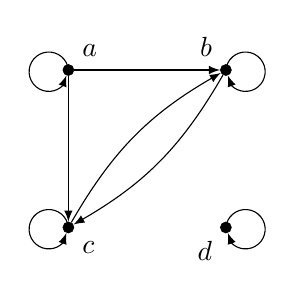
\begin{tikzpicture}[
	vertex/.style={ circle, draw, very thin, fill, inner sep=0pt, minimum size=4pt },
	vertexg/.style={ black!40!white, circle, draw, very thin, fill, inner sep=0pt, minimum size=4pt },
	vertexo/.style={ circle, draw, very thin, inner sep=0pt, minimum size=4pt }
]

\node at (2,-2) (d) [vertex,label=below left:{$d$}] {};
\node at (0,-2) (c) [vertex,label=below right:{$c$}] {};
\node at (2,0) (b) [vertex,label=above left:{$b$}] {};
\node at (0,0) (a) [vertex,label=above right:{$a$}] {};
\draw[-latex] (a) to (b);
\foreach \p in {a,c} \draw[-latex] (\p) arc (5:315:0.25cm) to (\p);
\foreach \p in {b,d} \draw[-latex] (\p) arc (175:-135:0.25cm) to (\p);
\draw[-latex] (a) to (c);
\draw[-latex] (c) to [out=60,in=210] (b);
\draw[-latex] (b) to [out=240,in=30] (c);

\end{tikzpicture}
